%-*- coding: utf-8 -*-
\subsubsection{Élaboration automatique des menus}
\begin{figure}[H]
\label{MenuGen}
  \centering
      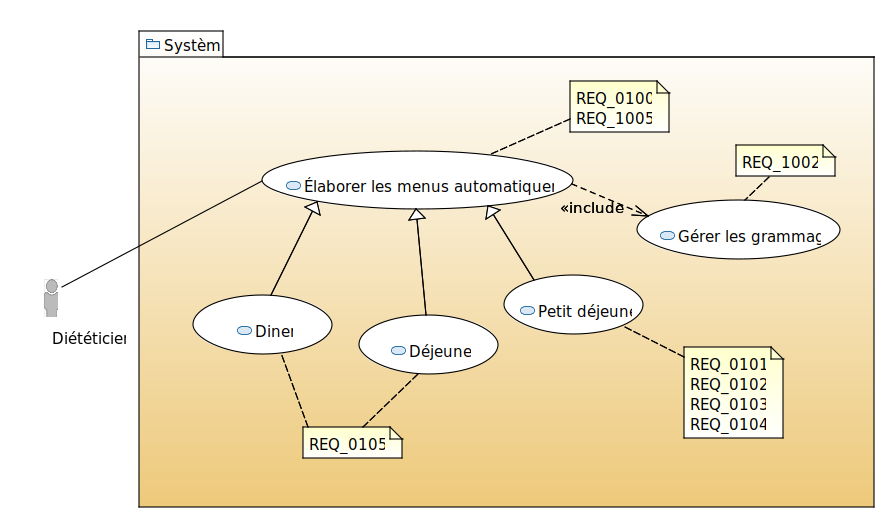
\includegraphics[width=1.00\textwidth]{../../CasDUtilisations/MenuGen/MenuGen.png} %
\caption{Élaboration automatique des menus}
\end{figure}

\begin{description}
\item[Nom:] Élaboration automatique des menus.
\item[ID:] UC300
\item[Description:] Permet l'élaboration automatique des menus.
\item[Auteur:] Jean-Félix BENITEZ.
\item[Date:] 07/05/2017
\item[Acteurs:] Diététiciens.
\item[Pré-Conditions:] Le diététicien s'est connecté au système.
\item[Scénario principal:]
  \begin{enumerate}
  \item Le diététicien sélectionne le groupe de patients pour lequel il veut générer les menus,
  \item ensuite il lance l'élaboration automatique.
  \item l'élaboration automatique ce déroule en prenant en compte les grammages.
  \end{enumerate}
\item[Scénario alternatif:] Aucun.
\item[Post-Conditions:] Les menus sont générés.
\end{description}
